%-----------------------Homework------------------------------------
%-------------------Arman Shokrollahi---------------------------------

\documentclass[a4 paper]{article}
% Set target color model to RGB
\usepackage{tikz}
\usepackage{amsfonts}
\usepackage{amsthm}
\usepackage{amsmath}
\usepackage{amssymb}
\usepackage{comment}
\usepackage{algorithmic}
\DeclareMathOperator{\st}{\backepsilon^{'}}
\usetikzlibrary{decorations.text,calc,arrows.meta}
\usetikzlibrary{automata,positioning}% Set target color model to RGB
\input{preamble3.tex}


\begin{document}
%%%%%%%%%%%%%%%%%%%%%%%%%%%%%%%%%%%%%%%%%%%%%%%%%%%%%%%%
%ADD ACADEMIC YEAR, YOUR DATA
\homework{Coursework}{20XX/20XX}{WRITE YOUR SURNAME}{WRITE YOUR FIRST NAME}{WRITE YOUR ID NUMBER}%{XX$^{\mathbf{th}}$ Month 20XX at 5PM (GMT/BST)}{XX}
%%%%%%%%%%%%%%%%%%%%%%%%%%%%%%%%%%%%%%%%%%%%%%%%%%%%%%%%


%\begin{center}\rule{\textwidth}{0.4pt}\end{center}

%\begin{center}\textbf{\textit{Answer all FIVE questions}
%}\end{center}

\vspace{5mm}
\problem{1}

This is how an Automaton is drawn

\begin{center}
\begin{tikzpicture}[shorten >=2pt,node distance=3cm,on grid,auto] 
   \node[state, initial] (A)   {$A$}; 
        \node[state, accepting] (B) [right =of A] {$B$};
        \node[state, accepting] (C) [right =of B] {$C$};
 \node[state, accepting] (D) [below =of A] {$D$};
  \node[state, accepting] (E) [right =of D] {$E$};
    \node[state] (F) [right =of E] {$F$};
  \node[state, accepting] (G) [above right=of C] {$G$};
    \node[state, accepting] (H) [below =of E] {$H$};

   %\node[state] (q_1) [above right=of q_0] {$q_1$}; 
%   \node[state] (B) [above=of A] {$DE$};
  %   \node[state] (q2) [below =of s1] {$q_2$};
  %  \node[state] (q3) [right =of s2] {$q_3$};
  %  \node[state] (q4) [above =of q3] {$q_4$};
    \path[->] 
    (G)  edge [loop above] node {$1$} ()
     (H)  edge [loop below] node {$\epsilon$} ()
    (F)  edge [loop right] node {$0,1$} ()
    (A) edge [above] node  {$0$} (B)
    (A) edge [left] node  {$1$} (D)
     (B) edge [above] node  {$0$} (C)
     (D) edge [above] node  {$\epsilon$} (E)
      (E) edge [above] node  {$0,1$} (F)
      (C) edge [left] node  {$0,1$} (F)
      (D) edge [bend right, left] node  {$1$} (H)
      (H) edge [bend right, right] node  {$0$} (F)
      (B) edge [bend left, above] node  {$1$} (G)
      (G) edge [bend left] node  {$0$} (F)
    ;
   %         (q1) edge [bend left, right] node  {$b$} (q2)
   %         (q2) edge [bend left, left] node  {$b$} (q1)
%            (q2) edge [below] node  {$a$} (q3)
 %           (q3) edge [bend left, left] node  {$a$} (q4)
  %          (q4) edge [bend left, right] node  {$a$} (q3)
   %         (q4) edge [above] node  {$b$} (q2);
\end{tikzpicture}
\end{center}

\noindent and a function of transitions is a table of the type

 \begin{center}
$\delta$: \begin{tabular}{c|c|c}
    & $0$ & $1$\\
\hline
    $A$ & $A,B$ & $B,C$ \\
    $B$ & $\emptyset$& $B,C$ \\
    $C$ &  $\emptyset$   & $\emptyset$ 
\end{tabular}
\end{center}

\begin{flushright}
\boxed{\textbf{20 marks}}
\end{flushright}

\newpage
\vspace{5mm}
\problem{2}

The table to check the equivalence of two Automata is of the type 

\begin{center}
\begin{tabular}{c|c|c}
    &$a$&$b$\\
\hline    
$s_1,q_1$  & $s_1,q_1$ & \colorbox{yellow}{$s_2,q_2$}\\
     & \textcolor{orange}{\textbf{FS, FS}}&\textcolor{blue}{\textbf{IS, IS}} \\
     \hline
$s_2,q_2$ &\colorbox{yellow}{$s_3,q_3$} &$s_1,q_1$\\
& \textcolor{orange}{\textbf{FS, FS}}  & \textcolor{blue}{\textbf{IS, IS}}\\
\hline
$s_3,q_3$ &\colorbox{yellow}{$s_2,q_4$} &$s_3,q_3$\\
& \textcolor{blue}{\textbf{IS, IS}}  & \textcolor{blue}{\textbf{IS, IS}}\\
\hline
$s_2,q_4$ &$s_3,q_3$ &$s_1,q_1$\\
& \textcolor{blue}{\textbf{IS, IS}} &\textcolor{orange}{\textbf{FS, FS}}\\
\end{tabular}
\end{center}

A Turing Machine is also drawn as an Automaton

\begin{center}
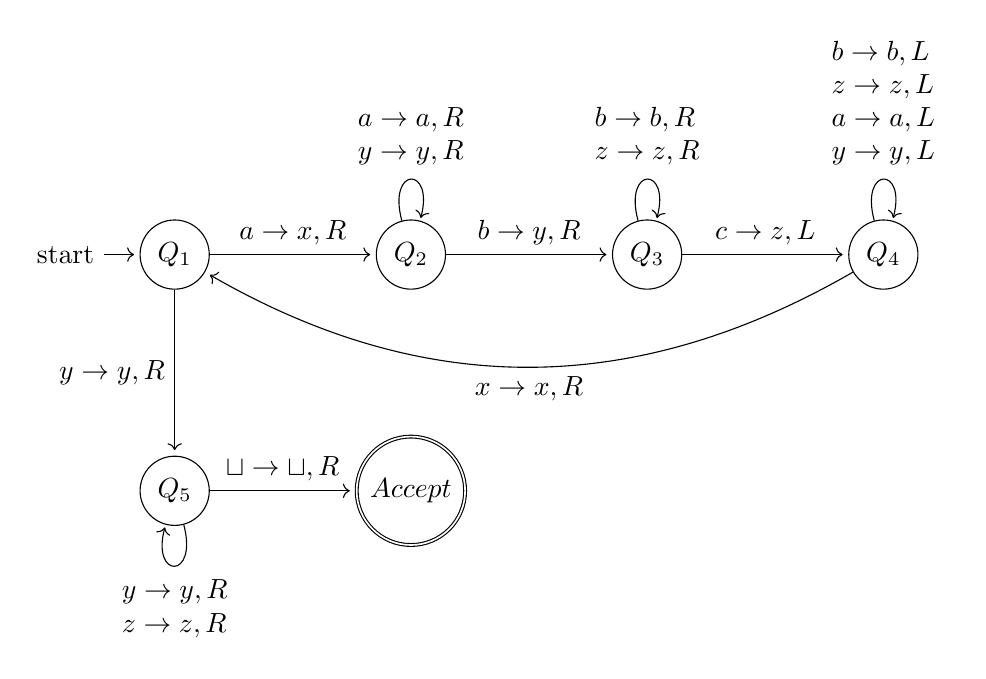
\begin{tikzpicture}[shorten >=2pt,node distance=3cm,on grid,auto] 
   \node[state,initial] (Q1)   {$Q_1$}; 
     \node[state] (Q2) [right=of Q1] {$Q_2$};
    \node[state] (Q3) [right=of Q2] {$Q_3$};
     \node[state] (Q4) [right =of Q3] {$Q_4$};
     \node[state] (Q5) [below =of Q1] {$Q_5$};
      \node[state, accepting] (Q6) [right =of Q5] {$Accept$};
    \path[->] 
    (Q2)  edge [loop above] node {$\begin{array}{l}
         a \to a, R  \\
         y \to y, R 
    \end{array}$} ()
     (Q3)  edge [loop above] node {$\begin{array}{l}
         b \to b, R  \\
         z \to z, R 
    \end{array}$} ()
      (Q4)  edge [loop above] node {$\begin{array}{l}
     b \to b, L  \\
         z \to z, L \\
         a \to a, L  \\
         y \to y, L 
    \end{array}$} ()
     (Q5)  edge [loop below] node {$\begin{array}{l}
         y \to y, R \\ 
           z \to z, R 
    \end{array}$} ()
     (Q1) edge  node {$a \to x, R$} (Q2)
          (Q2) edge  node {$b \to y, R$} (Q3)
           (Q3) edge  node {$c \to z, L$} (Q4)
           (Q4) edge [bend left] node {$x \to x, R$} (Q1)
           (Q1) edge [left] node {$y \to y, R$} (Q5)
           (Q5) edge [above] node {$\sqcup \to \sqcup, R$} (Q6);
\end{tikzpicture}
\end{center}


\begin{flushright}
\boxed{\textbf{20 marks}}
\end{flushright}

\newpage
\vspace{5mm}
\problem{3}

This is the notation to indicate a Grammar
\begin{equation*}
    G=\left(\lbrace S,A,B\rbrace, \lbrace a,b \rbrace, S, P  \right)
\end{equation*}
\noindent with production rules $P$ equal to
\begin{equation*}
    \begin{array}{l}
          S \to ASA|aB\\ 
          A\to B|S\\ 
          B\to b| \epsilon 
    \end{array}
\end{equation*}

\noindent and when transformations are made, we may indicate them as

\noindent \textbf{step 1: } Let us remove the null productions. 

\begin{center}
\begin{algorithmic}
\STATE \textbf{step 0 :}$W_0=\lbrace B\rbrace$
\STATE  \textbf{step 1 :}$W_1=\lbrace S, A, B\rbrace$
\STATE  \textbf{step 2 :}$W_2=\lbrace S, A, B\rbrace$
%\STATE  \textbf{step 3 :}$W_3=\lbrace S, A, B\rbrace$
\end{algorithmic}
\end{center} 
\noindent The set of nullable variables is $W=\lbrace S, A, B\rbrace$.

We may also present the algorithm in the following way 
\begin{equation*}
    \begin{array}{l}
         \textbf{step 0 :}W_0=\lbrace B\rbrace  \\
         \textbf{step 1 :}W_1=\lbrace S, A, B\rbrace\\ 
         \textbf{step 2 :}W_2=\lbrace S, A, B\rbrace
    \end{array}
\end{equation*}

\noindent \textbf{step 2: } Let us remove the unit productions. $\ldots$

\begin{flushright}
\boxed{\textbf{20 marks}}
\end{flushright}

\newpage
\vspace{5mm}
\problem{4}

A single state Pushdown Automaton is drawn like a Finite Automaton
\begin{center}
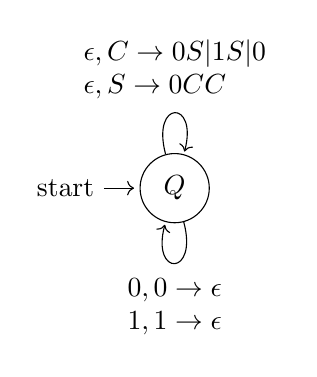
\begin{tikzpicture}[shorten >=2pt,node distance=3cm,on grid,auto] 
   \node[state, initial] (Q)   {$Q$}; 
    \path[->] 
        (Q)  edge [loop above] node {
        %\begin{equation*}
        $\begin{array}{l}
              \epsilon, C \to 0S|1S|0  \\
             \epsilon, S \to 0CC
        \end{array}$
        %\end{equation*}
        } ()
        (Q)  edge [loop below] node {
        % \begin{equation*}
        $\begin{array}{l}
        0, 0 \to \epsilon\\
        1, 1 \to \epsilon
         \end{array}$
        %\end{equation*}
        } ();
\end{tikzpicture}
\end{center}
 
This is an example of acceptance procedure by $\vdash$ notation

\begin{equation*}
    \begin{array}{l}
        \mathbf{\epsilon,S\to 0CC}: \left(Q,010000,\textcolor{blue}{S}\right)\vdash \left(Q,010000,\textcolor{red}{0CC}\right)\\
        
        \mathbf{0,0\to \epsilon}:\left(Q,\textcolor{blue}{0}10000,\textcolor{blue}{0}CC\right) \vdash \left(Q,10000,\textcolor{red}{CC}\right)\\
        
        \mathbf{\epsilon,C\to 1S}:\left(Q,10000,\textcolor{blue}{C}C\right)\vdash \left(Q,10000,\textcolor{red}{1S}C\right)  \\
        
        \mathbf{1,1\to \epsilon}:\left(Q,\textcolor{blue}{1}0000,\textcolor{blue}{1}SC\right) \vdash \left(Q,0000,\textcolor{red}{SC}\right)\\
        
         \mathbf{\epsilon,S\to 0CC}: \left(Q,0000,\textcolor{blue}{S}C\right)\vdash \left(Q,0000,\textcolor{red}{0CC}C\right)\\
        
         \mathbf{0,0\to \epsilon}:\left(Q,\textcolor{blue}{0}000,\textcolor{blue}{0}CCC\right) \vdash \left(Q,000,\textcolor{red}{CCC}\right)\\
        
        \mathbf{\epsilon,C\to 0}:\left(Q,000,\textcolor{blue}{C}CC\right)\vdash \left(Q,000,\textcolor{red}{0}CC\right)  \\
        
         \mathbf{0,0\to \epsilon}:\left(Q,\textcolor{blue}{0}00,\textcolor{blue}{0}CC\right) \vdash \left(Q,00,\textcolor{red}{CC}\right)\\
        
        \mathbf{\epsilon,C\to 0}:\left(Q,00,\textcolor{blue}{C}C\right)\vdash \left(Q,00,\textcolor{red}{0}C\right)  \\
        
         \mathbf{0,0\to \epsilon}:\left(Q,\textcolor{blue}{0}0,\textcolor{blue}{0}C\right) \vdash \left(Q,0,\textcolor{red}{C}\right)\\
        
        \mathbf{\epsilon,C\to 0}:\left(Q,0,\textcolor{blue}{C}\right)\vdash \left(Q,0,\textcolor{red}{0}\right)  \\
        
        \mathbf{0,0\to \epsilon}:\left(Q,\textcolor{blue}{0},\textcolor{blue}{0}\right) \vdash \left(Q,\epsilon,\textcolor{red}{\epsilon}\right)
    \end{array}
\end{equation*}


\begin{flushright}
\boxed{\textbf{20 marks}}
\end{flushright}

\newpage
\vspace{5mm}
\problem{5}

Theoretical questions may need inline equations that is $\sum_{i=1}^n x_i$ or a regular expression like $\left(a+b\right)^*$. A separate line equation is of the type
\begin{equation*}
    \left(a+b\right)^*
\end{equation*}

If a proof has to be provided then
\begin{proof}
Let us consider the following language $L\left(P\right)= \lbrace a \rbrace$, and equation
\begin{equation*}
    L\left(P^*\right)=\lbrace \epsilon, a, aa, aaa, \ldots \rbrace,
\end{equation*} 
\noindent which can make a point. Mathematical expressions can be of the type  $w \in L\left(QP^*\right)$ or something of the type 

\begin{equation*}
  \exists k \in \mathbb{N} \st  w \in L\left(QP^k\right)
\end{equation*}

\noindent or something or the type 
\begin{equation*}
  \forall x \in A \exists ! y \in B \st  \left(x, y \right) \in \mathcal{R}
\end{equation*}
\noindent with $f:A \to B$ and $\mathcal{R} \subseteq A \times B$.

\end{proof}

\begin{flushright}
\boxed{\textbf{20 marks}}
\end{flushright}

\end{document}